\chapter{NewSkillz Behaviour Framework}
\label{chap:rl}

\section{Introduction}
The work presented here describes the new behaviours framework for rUNSWift and is the combined effort of the following authors: Beth Crane, Jack Murray, Dan Padilha, Stephen Sherratt, and Alexander Whillas.

The \textit{NewSkillz} behaviour framework is a new implementation of the \verb!Python!-based control logic for the rUNSWift codebase. The new framework aims to replace the existing \verb!Python! skills by allowing for a much easier learning curve, easily understandable code, the removal of redundancy through abstraction, and less need for complex state transition models. Furthermore, the framework is abstracted in such a way that allows the same behaviour code to be run on the robots as well as in simulators with no modification required.

The 2012 behaviours were ported in a mostly-working state to the \textit{NewSkillz} framework, as a proof-of-concept. Examples in this section will stem from this proof-of-concept implementation.

As it required the effort of many authors, information about \textit{NewSkillz} is spread throughout various reports. In particular, more information about the integration with a simulator and the reasoning behind the framework can be found in the report by Crane and Sherratt.\cite{simulator} The focus of this section therefore is to provide a gentle introduction to implementing skills using the \textit{NewSkillz} framework, as well as documentation of its major features. Note that the terms \textit{behaviours} and \textit{skills} are used interchangeably throughout the text.

\section{Theory}

The behaviours framework is what controls the behaviour of the Nao robots when playing soccer. Specifically, this refers to all high-level decisions the robots must make. That is to say, the behaviours do \textit{not} define how a robot's body moves in order to make it walk, how the robot analyses a video image to find the ball, or how a robot communicates with its team-mates.

Instead, the behaviours framework defines how a robot decides whether to go for the ball or move to another position, whether to kick the ball or line itself up at a better angle, whether to dive for the ball as a goalie, and so on. This high-level decision-making requires rapid development during the competition in order to adapt to the opposing team strategies. For this reason, a high-level programming language (\verb!Python!) is used for the greatest ease of development.

The \textit{NewSkillz} framework differs from the 2012 skills framework in that it is not programmed explicitly as state-machines. Instead, the states arise from inherent properties of the framework while still being as simple to reason about. State is chosen through a tree-like structure of skills where each skill decides whether to \textit{delegate} its decision to another skill, or to perform some action in a \textit{tick}.

The skill tree can therefore be thought as a form of decision tree or state-machine. Each node in the tree is expected to delegate a decision down to a node below it. Leaf nodes -- those which do not wish to delegate -- are required to therefore perform some sort of action in the real world, such as kick the ball.

To better illustrate this concept, the skill tree for the proof-of-concept port of the 2012 skills is shown in Figure~\ref{fig:skill_tree}.

\begin{figure}[h]
\centering
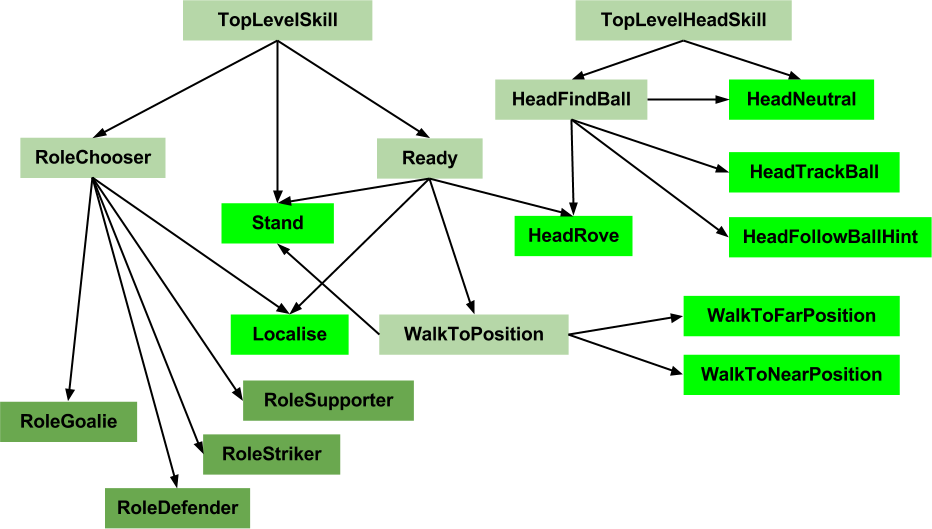
\includegraphics[width=0.9\textwidth]{img/skill_tree.png}
\caption{Tree of the proof-of-concept port of the 2012 skills. Skills in bright green are leaf nodes (which must perform some action). Skills in dark green are un-expanded nodes (i.e. the skills they delegate to are not shown). An arrow from a skill represents a delegation to another skill.}
\label{fig:skill_tree}
\end{figure}

Notice that the tree contains two root nodes, being \texttt{TopLevelSkill} and \texttt{TopLevelHeadSkill}. This allows for decisions to be made for the body and head separately.

The skill tree system provides cleaner and less redundant code through the delegation mechanism. It is easy to imagine this by taking the state machine of the head as an example.

\section{Implementation}

\subsection{Codebase}

The rUNSWift codebase is split into the \verb!C++! backend and the \verb!Python! behaviours framework. The behaviours framework is run through the \texttt{Perception} thread (running at $30Hz$) in 

\texttt{runswift/robot/behaviour/python/PythonSkill.cpp}

This defines the \verb!C++! to \verb!Python! interface. It also ensures that \textbf{live-reload} for skills works, such that a robot can be left running in a crashed state, new skills synced to it, and it will simply continue running as if it had never crashed.

The \verb!Python! entry-point is located in

\texttt{runswift/image/home/nao/data/behaviours/cpp\_glue.py}

On every tick, \texttt{cpp\_glue} ticks both the \texttt{TopLevelSkill} and \texttt{TopLevelHeadSkill}. Because the body's \texttt{TopLevelSkill} is ticked \textit{after} the head, any skills in the body skill tree can choose to delegate to a skill in the head tree and thus \textbf{override} the head tree's actions.

\subsection{In Real Life (IRL)}

\subsubsection{Sense}

\subsubsection{Action}

\subsection{Skills}

The \texttt{Skill} class is the ``bread and butter'' of the \textit{NewSkillz} framework. This class abstracts away state transitions entirely from the programmer and provides the \texttt{IRL} to all skills automatically. The class also defines the argument-passing interface for skills.

Every skill in the skill tree is a subclass of \texttt{Skill}. \texttt{Skill} provides two functions: \texttt{tick} and \texttt{delegate}. When implementing a skill, exactly \textbf{one} of these functions must be overloaded, depending on whether the skill expects to \textit{delegate} its decision to another skill, or \textit{tick} an \texttt{IRL} Action.

\subsubsection{Tick}

\subsubsection{Delegate}

\subsection{Geometry}

\subsection{Debugging} 

All \verb!Python! runtime exceptions and errors are caught by \texttt{cpp\_glue}. \texttt{cpp\_glue} keeps watch on the skill-tree in order to print debug information about it, and catches all \verb!Python! exceptions in order to place the robot into ``Emergency mode''.

Under ``Emergency mode'', the robot stops all movement, flashes all its LEDs in random colours, and audibly requests to be picked up (for use in the competition). The stack trace produced by \verb!Python! is able to show the faulting skill as well as its parent skill (which delegated to it), but no further up the line. If a bigger stack trace is required, simply print out the skill name in the \texttt{tick} function of \texttt{Skill}.

Also, thanks to the live-reload functionality built into \texttt{cpp\_glue}, new skills can be pushed to the robot or even edited directly on the robot. Once a \verb!Python! file is modified on the robot, \textit{NewSkillz} reloads all skills and the robot continues from whatever state it was in (as the \texttt{Blackboard} maintains state which the \texttt{IRL} accesses).

\section{Results \& Evaluation}

A major advantage resulting from the \textit{NewSkillz} framework is the significant cut down in redundant code due to the abstraction of the \texttt{Blackboard} into the \texttt{IRL} API. By design, all skills have access to the \texttt{IRL}, and therefore to the \texttt{Blackboard} -- which needed to be passed around to everything in the 2012 framework. The standard \texttt{Skill} class also helps to abstract state transitions away, leaving much cleaner code.

\section{Future Work}

% TODO Tick locking
% TODO ncurses
% TODO Port the 2013 competition code

\section{Conclusion}
